\subsection{Ruang Kosong (\emph{Empty World})}
\label{subsec:lingkunganoutdoor}

Ruang kosong (\emph{empty world}) dibuat dengan menyusun \emph{file} SDFormat yang berisi objek paling dasar yang dibutuhkan oleh robot.
Ruangan virtual ini dibuat untuk memudahkan pengujian gerakan pada robot sehingga robot dapat bergerak secara bebas tanpa terhalang oleh \emph{obstacle} lain.

Seperti yang terlihat pada potongan kode \ref{lst:outdoorworldsdf},
  ruangan virtual ini terdiri atas sebuah objek pencahayaan yang berupa \emph{light element},
  dan dua buah \emph{include element} dengan \emph{path} \lstinline{model://ground_plane} dan \emph{path} \lstinline{model://dienen_robot}.
Kedua \emph{include element} tersebut digunakan untuk memasukkan model \emph{ground plane} yang sudah disediakan oleh Gazebo dan model robot yang telah dibuat sebelumnya di bagian \ref{sec:modelrobot}.

\lstinputlisting[
  language=XML,
  style=code,
  caption={Struktur SDFormat dari ruang kosong (\emph{empty world}).},
  label={lst:outdoorworldsdf}
]{kode/sdf/outdoor_world.xml}

Setelah \emph{file} SDFormat dibuat,
  hasil yang didapatkan setelah dijalankan pada simulator tampak seperti pada gambar \ref{fig:lingkunganoutdoor}.
Sesuai dengan susunan yang diisi pada \emph{file} SDFormat,
  tampak adanya model robot dengan objek \emph{ground plane} yang ada di bawah,
  sedangkan objek pencahayaan tampak dengan adanya bayangan dari robot dan gradasi warna cerah pada objek \emph{ground plane}.

\begin{figure}[ht]
  \centering
  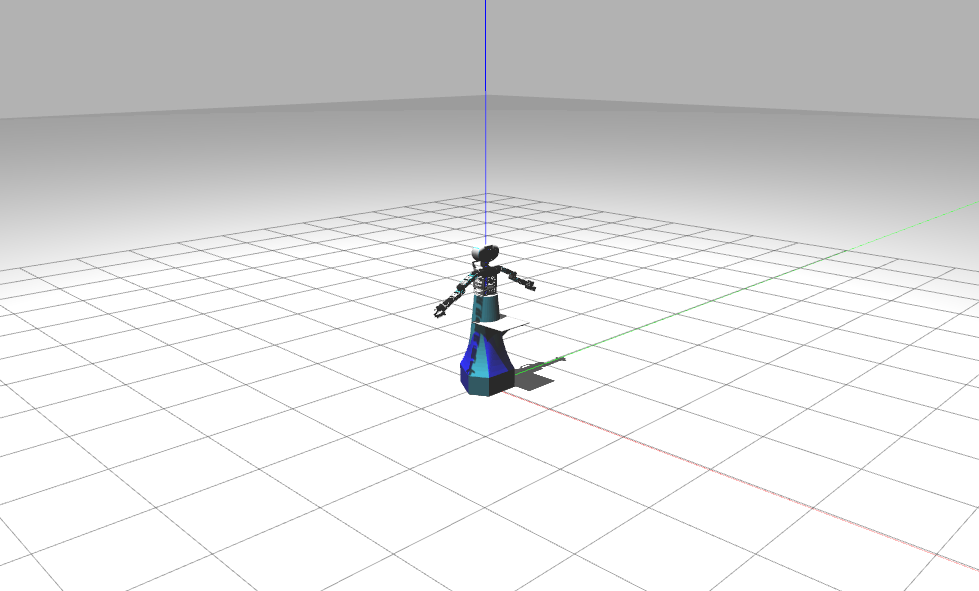
\includegraphics[scale=0.23]{gambar/lingkungan-outdoor.png}
  \caption{Tampilan ruang kosong (\emph{empty world}) pada Gazebo.}
  \label{fig:lingkunganoutdoor}
\end{figure}
